\documentclass[11pt]{article}
\usepackage{times}
\usepackage{fullpage}
\usepackage{url}
\usepackage{hyperref}
\usepackage{fancyhdr}
\usepackage{graphicx}
\usepackage{enumitem}
\usepackage{subcaption}
\usepackage{amsmath, amsfonts, amsthm, fouriernc}
\usepackage{IEEEtrantools}
\usepackage{parskip}

\pagestyle{fancy}
\addtolength{\headheight}{2em}
\addtolength{\headsep}{1.5em}
\lhead{\large{ME 2801}}

\usepackage{sectsty}
\sectionfont{\fontsize{12}{8}\selectfont}

\begin{document}

\begin{center}
  \Large{\bf{Assignment: Transfer Functions and Modeling}}
\end{center}

The textbook exercises, designated with the word ``Nise'', are from the ``Problems'' section at the end of Chapter~2 in \emph{Control System Engineering} by Norman Nise, 7th edition.

\textbf{Nise reading:}
\begin{itemize}[nosep]
  \item Chapter 2, Sections 2.5 and 2.6
  \item Appendix B, ch2p9--ch2p12
\end{itemize}

% ---------------------------------------------------------------
\section*{Inverse Laplace Transform of Functions}

\begin{enumerate}

\item Given the following Laplace transforms, find the corresponding time functions.  Use the MATLAB \texttt{residue} function for the partial fraction expansion.  You do not need to turn in your MATLAB scripts.
  \begin{enumerate}[label=\alph*)]
    \item $F(s) = \dfrac{s+5}{(s+2)(s^2+36)}$
    \item $G(s) = \dfrac{2}{s\,(s^2+s+16.25)}$
    \item $H(s) = \dfrac{1}{(s^2+9)(s^2+4s+1)}$
  \end{enumerate}

\end{enumerate}

% ---------------------------------------------------------------
\section*{Transfer Functions}

\begin{enumerate}[resume]

\item Nise 2.8

\item Nise 2.9

\end{enumerate}

% ---------------------------------------------------------------
\section*{Transfer Function Representation in MATLAB}

\begin{enumerate}[resume]

\item Consider each of the following transfer functions:
  \begin{enumerate}[label=\alph*)]
    \item $G(s) = \dfrac{3}{s^3 + 9s^2 + 20s}$
    \item $H(s) = \dfrac{10(s+2)}{s^2(s+4)(s+5)}$
  \end{enumerate}
  For each expression, illustrate (submit a snippet of MATLAB script) how you would generate the transfer function object in MATLAB using the two methods:
  \begin{itemize}[nosep]
    \item using the ratio of factors (the \texttt{zpk()} function)
    \item using the ratio of polynomials (the \texttt{tf()} function)
  \end{itemize}

\item Nise 2.13

  Note: the \texttt{roots} function can be used to find the roots of a polynomial.  For example, to find the roots of $s^2 + 5s + 30$ we could do the following\ldots
\begin{verbatim}
>> roots([1 5 30])
ans =
  -2.5000 + 4.8734i
  -2.5000 - 4.8734i
\end{verbatim}

\end{enumerate}

% ---------------------------------------------------------------
\section*{USV Model}

% CLAUDE: Put into a figure environment for proper LaTeX formatting.
\begin{figure}[h!]
  \centering
  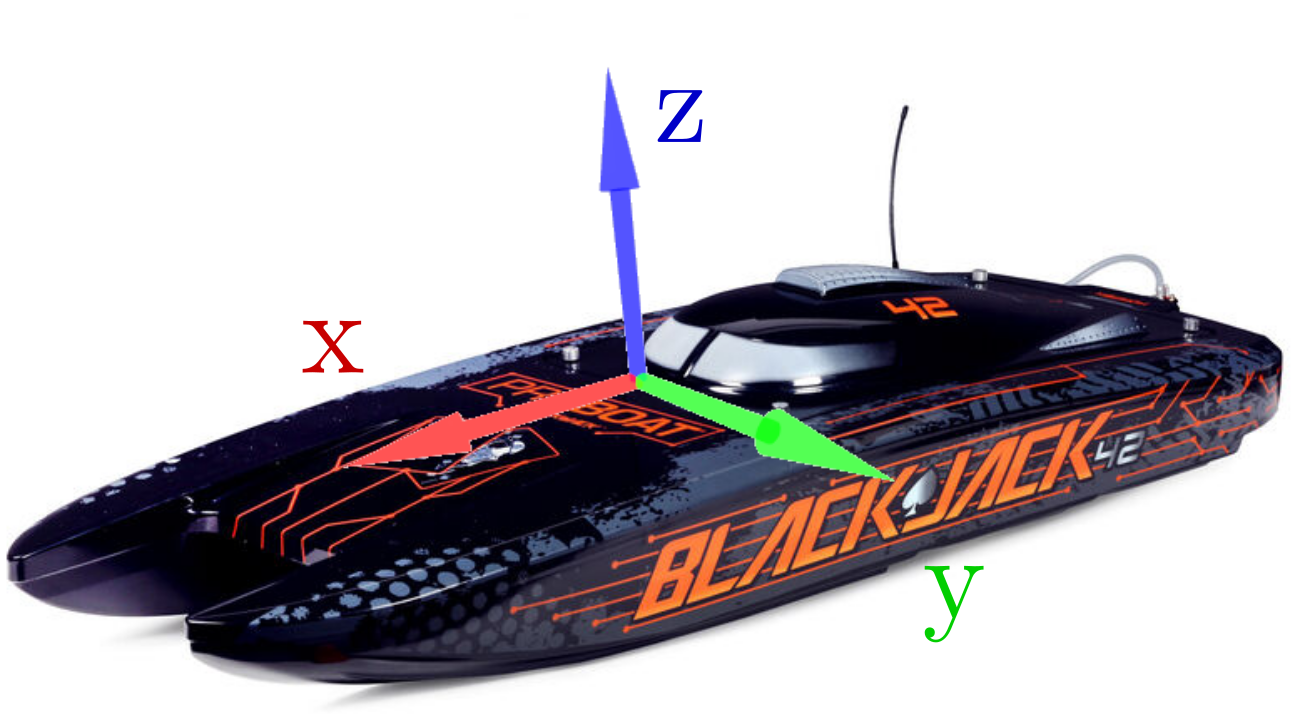
\includegraphics[width=0.6\linewidth]{images/blackjack_cs.png}
  \caption{Small unmanned surface vessel (USV).}
  \label{fig:blackjack_cs}
\end{figure}

Consider the small unmanned surface vessel (USV) in Figure~\ref{fig:blackjack_cs}.  The vessel is approximately 1.1\,m long with a mass of 5\,kg.  It has a single  propeller on the centerline, which produces a thrust force $F(t)$ [N] along the body $x$-axis, and a single stern rudder, which produces a yaw moment $N(t)$ [N$\cdot$m] about the body $z$-axis.

The vessel has six degrees of freedom: three translations (surge, sway and heave) and three rotations (roll, pitch and yaw).  Because the propeller is on the centerline, we treat the two inputs as decoupled: thrust controls forward speed, and the rudder controls heading.  We model only two scalar motions:
\begin{itemize}[nosep]
  \item Surge velocity $v_x(t)$ [m/s], forward velocity along the body $x$-axis.% CLAUDE: change velocity notation to v_x(t), etc. 
  \item Yaw rate $r(t) = \dot{\psi}(t)$ [rad/s], where $\psi(t)$ [rad] is the heading angle.
\end{itemize}

\begin{enumerate}[resume]

\item Consider the surge direction only.  Find the equation of motion in the surge (+$x$) direction with the following assumptions:
  \begin{itemize}[nosep]
    \item The total inertia (rigid body plus added mass) of the vessel in the surge direction is $m = 5.0$ [kg].
    \item The total drag on the vessel is linearly related to surge velocity, with a coefficient of $b_u = 8.0$ [N$\cdot$s/m].
    \item The only other force in the surge direction is the propeller thrust $F(t)$ [N].
  \end{itemize}

\item Consider the scenario where the vessel starts at rest with no input.  At time zero the propeller thrust is set to a constant $F(t) = 12.0$ [N].
  \begin{itemize}[nosep]
    \item Using Laplace transforms, solve the equation of motion to find the surge velocity $v_x$ as a function of time.
    \item Using the expression obtained, plot the time response of the surge velocity $v_x$ vs time $t$. Include labels and units on the axes.
    \item Indicate the ``steady-state speed'' of the vessel?
    \item How long does it take for the vessel to reach 95\% of the steady-state speed?  (An estimate from the graph is sufficient.)
  \end{itemize}

\item Find the transfer function for the surge direction where the input is the thrust $F$ and the output is the surge velocity $v_x$.

\item Next, consider the yaw direction only.  Find the equation of motion in the yaw direction with the following assumptions:
  \begin{itemize}[nosep]
    \item The total inertia (rigid body plus added inertia) of the vessel about the yaw axis is $I = 0.8$ [kg$\cdot$m$^2$].
    \item The drag moment on the vessel is linearly related to yaw rate, with a coefficient of $b_r = 1.2$ [N$\cdot$m$\cdot$s/rad].
    \item The only other moment about the yaw axis is the rudder moment $N(t)$ [N$\cdot$m].% CLAUDE: Change this so that the input is the rudder deflection rather than the rudder moment.  Explain this a reasonable approximation for small angles at a constant forward speed.
  \end{itemize}

\item Find the transfer function for the yaw direction where the input is the rudder moment $N(t)$ and the output is the yaw rate $r(t)$.

\item Find the transfer function for the yaw direction where the input is the rudder moment $N(t)$ and the output is the heading angle $\psi(t)$.

\item Consider the scenario where the vessel starts with zero yaw rate and zero heading.  At time zero the rudder moment is set to a constant $N(t) = 0.6$ [N$\cdot$m].
  \begin{itemize}[nosep]
    \item Use the final value theorem to find the steady-state yaw rate.
    \item Apply the final value theorem to the heading angle $\psi(t)$.  Does the result make physical sense?  Explain what the vessel is doing as $t \to \infty$.
  \end{itemize}

\end{enumerate}

\end{document}
